\documentclass[preprint,12pt]{elsarticle}
\usepackage{amsmath,amssymb,amsthm,amsfonts}
\usepackage{stix}
\usepackage{booktabs,graphicx,xcolor,float,array}
\usepackage[colorlinks=true,linkcolor=blue,citecolor=blue,urlcolor=blue]{hyperref}
\newtheorem{result}{Result}
\theoremstyle{remark}
\newtheorem{remark}{Remark}
\newfloat{algorithm}{tbp}{loa}
\floatname{algorithm}{Algorithm}
\newcommand{\todo}[1]{\textcolor{red}{\textbf{[TODO: #1]}}}

\newcommand{\step}[1]{\par\noindent\hangindent=1.5em\hangafter=1\textbf{Step #1.}\ }
\setlength{\emergencystretch}{2.5em}
\newcommand{\repo}{\url{https://github.com/mossaiby/iHaar}}
\newcommand{\archive}{\url{https://github.com/mossaiby/iHaar/releases/tag/v1.1}}
\journal{Computer Methods in Applied Mechanics and Engineering}

\begin{document}
\begin{frontmatter}
\title{Fast solvers on arbitrary grids for Haar wavelet collocation:
sharp-interface phase-field computations and adaptive elastostatics}

\author[inst1]{Farshid Mossaiby\corref{cor1}}
\ead{mossaiby@eng.ui.ac.ir}
\cortext[cor1]{Corresponding author}
\affiliation[inst1]{organization={Department of Civil Engineering, University of Isfahan},
            city={Isfahan}, postcode={81744-73441}, country={Iran}}

\begin{abstract}
The Haar wavelet collocation method (HWCM) is popular in engineering because it is easy to derive and
to program. In two and three dimensions, however, it is usually solved through large dense matrices, it
is limited to second-order accuracy, and it offers no stability guarantees for nonlinear problems. We
show that these limitations disappear when the method is written in terms of nodal values. An exact
three-term relation turns the dense HWCM matrices into tridiagonal ones, and we prove that the resulting
second-derivative operator has real, simple and nonpositive eigenvalues on every grid, uniform or
graded. This guarantee means that fast diagonalization, the fastest structured solver available, is always well
defined, including on grids generated by adaptive refinement. Its numerical reliability is a separate
matter. It was backward stable on random and deliberately adversarial grids, and an inexpensive check
switches to a slower, backward-stable solver if ever needed. On uniform grids, a correction that costs nothing
extra raises the accuracy to fourth order. Building on this, we present Allen--Cahn and Cahn--Hilliard
solvers that conserve mass exactly and satisfy a modified-energy law for any time step, and that resolve interfaces
only about two grid nodes wide on $1024^2$ grids. We also present a plane elastostatics solver with
prescribed displacements and tractions, whose number of iterations does not grow with the mesh, and
whose automatic refinement recovers the optimal convergence rate at crack-like corner singularities.
Against biquadratic finite elements on the same grids and with the same type of solver, the method reaches
a given accuracy with a quarter of the unknowns, which in our implementation saved time and memory as well. We also state where the method is not the best choice. The code that reproduces every result is
openly available.
\end{abstract}

\begin{keyword}
Haar wavelet collocation \sep fast diagonalization \sep graded grids \sep Cahn--Hilliard \sep
sharp interfaces \sep corner singularities \sep adaptive refinement
\end{keyword}
\end{frontmatter}

%==========================================================================
\section{Introduction}
%==========================================================================
The Haar wavelet collocation method (HWCM)~\cite{chen1997haar,lepik2005numerical,lepik2011solving,lepik2014book}
is widely used in applied mechanics for beams, plates, shells and functionally graded
structures~\cite{majak2015accuracy,majak2015convergence,majak2018higher}. The highest derivative of the
unknown is expanded in Haar functions, the lower derivatives follow by exact integration, and the
equation is enforced at cell midpoints. Higher-order variants~\cite{majak2018higher,ratas2021solving} and
graded grids based on non-uniform Haar functions~\cite{dubeau2004nonuniform,lepik2008nonuniform,oruc2019nonuniform}
are available. In two dimensions, however, all equations are usually assembled into one dense matrix of
size $N^2\times N^2$, which becomes impractical beyond about $64\times64$ cells. Graded grids must be
designed by hand, and nonlinear time-dependent problems have no stability guarantees.

In terms of nodal values, HWCM is midpoint quadratic-spline collocation
(QSC)~\cite{houstis1988quadratic,christara1994quadratic,christara2006optimal}, and it uses the same
functions as quadratic isogeometric collocation~\cite{auricchio2010isogeometric,schillinger2013isogeometric}.
For structured grids, the fastest solver family is fast diagonalization~\cite{lynch1964direct}. It
reduces two- and three-dimensional problems to dense matrix products, which run efficiently on CPUs and
GPUs, but it requires each one-dimensional operator to be diagonalizable with real eigenvalues. For
symmetric finite-element and isogeometric Galerkin operators this is automatic~\cite{sangalli2016isogeometric}.
Collocation operators are generally not symmetric, and for them the property has to be proved. For
Hermite-cubic orthogonal spline collocation it is known~\cite{dyksen1987tensor,sun1999spectral}, and it
underlies the matrix decomposition algorithms of Bialecki and Fairweather~\cite{bialecki1995matrix,bialecki2011matrix}.
For QSC, fast solvers exist on uniform grids~\cite{christara2002fast}. To our knowledge, the property has
not been established for midpoint QSC, equivalently nodal HWCM, on arbitrary graded grids.
Without a guarantee, fast diagonalization on adaptively refined grids could fail.

This paper closes that gap and builds on it. Our central result is that, on every grid, the HWCM
second-derivative operator has real, simple and nonpositive eigenvalues (Result~\ref{thm:spectrum}). We
then use this guarantee in three engineering settings. The first is fast solution on arbitrary graded
grids. The second is Allen--Cahn and Cahn--Hilliard computations with very thin interfaces, which
conserve mass exactly and are energy-stable. The third is elastostatics with traction boundaries and
automatic refinement at corner singularities. Table~\ref{tab:closest} compares the method with the
closest existing approaches. The results are stated in the main text together with their practical
meaning; formal statements and proofs are given in Part~A of the Supplementary Material. The code is
available at \repo.

\begin{table}[t]\centering\footnotesize
\caption{Comparison with the closest spline-collocation approaches, to the best of our knowledge. ``Spectrum'' refers to the one-dimensional collocation operator used by fast diagonalization or matrix decomposition.}\label{tab:closest}
\begin{tabular}{p{2.2cm}p{2.6cm}p{2.0cm}p{3.4cm}p{2.6cm}}
\toprule
Method & Trial space and collocation points & Grids & Spectrum & Fast solver\\
\midrule
Classical HWCM~\cite{lepik2011solving,oruc2019nonuniform} & integrated Haar ($C^1$ quadratics); midpoints & uniform or a~priori graded & not analysed & none (dense $N^2\times N^2$ solve)\\
Hermite-cubic OSC~\cite{dyksen1987tensor,sun1999spectral,bialecki1995matrix} & $C^1$ cubics; two Gauss points per cell & partitions as in the cited works & real, distinct eigenvalues established & matrix decomposition (MDA), FFT on uniform grids\\
QSC~\cite{houstis1988quadratic,christara2002fast,christara2006optimal} & $C^1$ quadratics; midpoints (optimal variants perturbed) & uniform; non-uniform analysed for convergence & symmetric with trigonometric eigenvectors on uniform grids & FFT and MDA on uniform grids\\
Quadratic IGA collocation~\cite{auricchio2010isogeometric,schillinger2013isogeometric,delorenzis2015isogeometric} & B-splines; Greville or superconvergent points & arbitrary knots; local refinement & not established for collocation; Galerkin pencils symmetric~\cite{sangalli2016isogeometric} & direct or Krylov; FDM for the Galerkin counterpart\\
This work & $C^1$ quadratics; midpoints & arbitrary graded tensor grids & real, simple, nonpositive on every grid (Result~\ref{thm:spectrum}) & FDM on any tensor grid, with a safeguard; DCT/DST on uniform grids\\
\bottomrule
\end{tabular}
\end{table}

%==========================================================================
\section{The method}\label{sec:method}
%==========================================================================
\subsection{Nodal form of Haar wavelet collocation}
Let $a=t_0<t_1<\dots<t_N=b$ be the grid, with cells of width $h_k$, midpoints $m_k$, and midpoint
spacings $d_k=(h_k+h_{k+1})/2$. HWCM expands $u''$ in Haar functions and integrates twice. On a given
grid, the Haar functions span exactly the functions that are constant on each cell, so the Haar
coefficients carry the same information as the cell values $c_k$ of $u''$. Integrating twice gives
piecewise quadratics with continuous slopes, which are quadratic splines. We use the values $U_k$ at the
cell midpoints, which are the HWCM collocation values, as unknowns.

\begin{result}[Three-term identity]\label{thm:identity}
For every quadratic spline on the grid, the nodal values and the cell values of $u''$ are related by
\begin{equation}\label{eq:interior}
\frac{U_{k+1}-U_k}{d_k}-\frac{U_k-U_{k-1}}{d_{k-1}}
=\frac{h_{k-1}^2}{8d_{k-1}}c_{k-1}+\Big(h_k-\frac{h_k^2}{8d_{k-1}}-\frac{h_k^2}{8d_k}\Big)c_k+\frac{h_{k+1}^2}{8d_k}c_{k+1},
\end{equation}
with modified first and last rows that contain the boundary data, either a prescribed value
(Eq.~\eqref{eq:dirrow}) or a zero slope (Eq.~\eqref{eq:neurow}):
\begin{align}
\frac{U_2-U_1}{d_1}-\frac{2(U_1-g_0)}{h_1}&=\Big(\frac{3h_1}{4}-\frac{h_1^2}{8d_1}\Big)c_1+\frac{h_2^2}{8d_1}c_2,\label{eq:dirrow}\\
\frac{U_2-U_1}{d_1}&=\Big(h_1-\frac{h_1^2}{8d_1}\Big)c_1+\frac{h_2^2}{8d_1}c_2.\label{eq:neurow}
\end{align}
In matrix form $LU+b=Ac$, with tridiagonal $L$ and $A$. The collocation problem always has a unique
solution.
\end{result}

The second derivative at the nodes is therefore $c=D_2U+(\text{boundary terms})$, with $D_2=A^{-1}L$.
Instead of the dense integration matrices of classical HWCM, only two tridiagonal matrices need to be
assembled. Slopes follow in closed form as well, which gives the first-derivative matrix $D_1$ and the
end slopes needed for traction conditions (Algorithm~1).

\begin{algorithm}[t]\small\hrule\smallskip
\noindent\textbf{Algorithm 1: one-dimensional operators} (\texttt{ihaar/core.py}, class \texttt{Grid1D}).
Input: knots $t_0<\dots<t_N$ and the type of each end (value prescribed, or zero slope).
\step{1} Compute $h_k$, $m_k$ and $d_k$, and assemble the tridiagonal matrices $L$ and $A$ from~\eqref{eq:interior}--\eqref{eq:neurow}.
\step{2} Factorize $A$ (tridiagonal LU) and form $D_2=A^{-1}L$ and the boundary vectors $e_i=A^{-1}b_i$.
\step{3} Form the first-derivative matrix $D_1=\mathbf 1r^{\mathsf T}+TD_2$, where $T_{kj}=h_j$ for $j<k$, $T_{kk}=h_k/2$, and $r$ encodes $\sigma_0$.
\step{4} Form the end slopes $s'(a)=\sigma_0$ and $s'(b)=\sigma_0+\sum_kh_kc_k$ as row vectors, for traction conditions.
\smallskip\hrule
\end{algorithm}

\subsection{Main result: the fast solver always works}
\begin{result}[Spectrum on every grid]\label{thm:spectrum}
On every grid, and whether a value or a zero slope is prescribed at each end, $D_2=A^{-1}L$ has real,
distinct and nonpositive eigenvalues. It is therefore diagonalizable with a real eigenvector matrix
$V$. Zero is an eigenvalue only when the slope vanishes at both ends.
\end{result}

On uniform grids $D_2$ is symmetric, and the result is easy. On graded grids $D_2$ is not symmetric, and
the result rests on a less familiar property. The matrix $A$ and the inverse of $-L$ are totally
nonnegative, meaning that all their minors are nonnegative. Their product then belongs to the class of
oscillation matrices studied by Gantmacher and Krein for vibrating mechanical
systems~\cite{gantmacher2002oscillation}, whose eigenvalues are always real and distinct. For the engineer, the consequence is that fast diagonalization is always defined, whatever grid the
refinement produces. Result~\ref{thm:spectrum} does not bound the conditioning of $V$, however, so the
code checks the accuracy of every solve through its residual and falls back to the backward-stable
Bartels--Stewart algorithm if needed. We also tested the accuracy directly (Section~\ref{sec:robust}). The same eigenvectors diagonalize every operator of the form
$\alpha D_2^x\oplus\beta D_2^y+\gamma I$ in two dimensions, and likewise in three.

\subsection{Uniform grids: cosine transforms, fourth order and mass conservation}
\begin{result}[Uniform grids]\label{thm:fourth}
On a uniform grid, $D_2=\frac{8}{h^2}\delta^2(8I+\delta^2)^{-1}$, where $\delta^2$ is the usual three-point
second difference. It is symmetric and diagonalized by the discrete cosine (zero slope) or sine
(prescribed values) transform. The corrected operator
\begin{equation}\label{eq:D24}
D_2^{(4)}=D_2+\tfrac{h^2}{24}D_2^2
\end{equation}
has the same eigenvectors and is fourth-order accurate for zero-flux and periodic problems.
\end{result}

\begin{result}[Exact mass conservation]\label{prop:mass}
With zero slope at both ends, the weighted sum $\sum_kh_kU_k$ is conserved by $D_2$ on any grid. On a
uniform grid, it equals the exact integral of the spline.
\end{result}

Plain HWCM has half the error constant of the standard three-point difference, so it is about twice as
accurate on the same grid. The fourth-order correction costs nothing, because in the transform domain it
only changes the eigenvalues.

%==========================================================================
\section{Fast solvers in two and three dimensions}\label{sec:tensor}
%==========================================================================
On a rectangle, the unknowns form a matrix $U_{ij}$, and the one-dimensional operators act along the grid
lines: $U_{xx}=D_2^xU$ and $U_{yy}=U(D_2^y)^{\mathsf T}$, plus boundary terms. An equation such as
$\alpha u_{xx}+\beta u_{yy}+\gamma u=f$ becomes a Sylvester matrix equation. With the eigendecompositions
$D_2^x=V_x\Lambda_xV_x^{-1}$ and $D_2^y=V_y\Lambda_yV_y^{-1}$, which exist by Result~\ref{thm:spectrum},
its solution is
\begin{equation}\label{eq:fdm}
U=V_x\Big[\big(V_x^{-1}\tilde FV_y^{-\mathsf T}\big)\oslash\big(\alpha\lambda^x_i+\beta\lambda^y_j+\gamma\big)_{ij}\Big]V_y^{\mathsf T},
\end{equation}
where $\oslash$ denotes entrywise division. This takes four dense matrix products after a one-time
eigendecomposition. In three dimensions the cost is $O(N^4)$, and on uniform grids fast cosine
transforms reduce it to $O(N^d\log N)$. All operations are dense matrix products, fast transforms or
pointwise operations. The code takes the array library (NumPy or CuPy) as a parameter, so the same code
runs on CPUs and GPUs.

%==========================================================================
\section{Phase-field solvers}\label{sec:pf}
%==========================================================================
We solve the Allen--Cahn (AC) and Cahn--Hilliard (CH) equations with zero-flux boundaries,
$u_t=-\mathcal G\mu$, $\mu=-\varepsilon^2\Delta u+u^3-u$, with $\mathcal G=I$ for AC and $\mathcal G=-\Delta$
for CH. The parameter $\varepsilon$ sets the interface thickness. Across an equilibrium interface
$u\approx\tanh(d/\sqrt2\varepsilon)$, where $d$ is the distance to the interface. With $K$ the discrete
$-\Delta$, $\bar u=2u^n-u^{n-1}$, and a scalar auxiliary variable $r$~\cite{shen2018scalar}, the
stabilized SAV-BDF2 scheme reads
\begin{align}
\frac{3u^{n+1}-4u^n+u^{n-1}}{2\Delta t}&=-G\mu^{n+1},\qquad
\mu^{n+1}=\varepsilon^2Ku^{n+1}+S(u^{n+1}-\bar u)+r^{n+1}\bar b,\label{eq:sav1}\\
3r^{n+1}-4r^n+r^{n-1}&=\tfrac12\langle\bar b,3u^{n+1}-4u^n+u^{n-1}\rangle_h,\label{eq:sav2}
\end{align}
where $\bar b=f(\bar u)/\sqrt{E_1(\bar u)+C}$ is the scaled nonlinearity and $S\ge0$ a stabilization
constant. Each step costs one forward and one inverse transform (Algorithm~2). The scheme works in three dimensions
as well; a three-dimensional accuracy test is reported in Table~S19.

\begin{result}[Mass and energy]\label{thm:energy}
On a uniform grid, for every time step and every $S\ge0$, the scheme has a unique solution, the CH scheme
conserves the discrete mass exactly, and a modified energy never increases.
\end{result}

It is important to know what this guarantee does not cover. It concerns a \emph{modified} energy. That
the physical energy decreases, that $u$ stays bounded, and that interfaces move correctly are separate
properties, which we only observe in our tests. For thin interfaces they need stabilization: with
$S=0$, a computation with $\varepsilon=0.0015$ produced values of $|u|$ around 30 to 70 while the
modified energy kept decreasing, whereas $S=4$ kept $|u|\le1.04$ (Table~\ref{tab:savstab}). A systematic study (Table~S18) shows that the smallest $S$ that keeps the ratio $\xi=r/\sqrt{E_1+C}$
close to one is the most accurate: $S\approx1$ to 2 for time steps up to $\varepsilon^2$, and 2 to 4 for
larger steps. Even then, steps much larger than $\varepsilon^2$ give wrong interface motion, so $\xi\approx1$
does not replace checking the time step. These are empirical recommendations, not proved thresholds.

\begin{algorithm}[t]\small\hrule\smallskip
\noindent\textbf{Algorithm 2: one SAV-BDF2 time step} (\texttt{ihaar/phasefield.py}).
Precomputed: the transform $\mathcal T$ (DCT-II, or the eigenvectors $V$), the symbols $\hat\lambda$ of
$-K$, $\hat G=1$ (AC) or $\hat\lambda$ (CH), and $\hat S_2=3+2\Delta t\,\hat G(\varepsilon^2\hat\lambda+S)$.
Stored from previous steps: $\hat u^n$, $\hat u^{n-1}$, $u^n$, $u^{n-1}$, $r^n$, $r^{n-1}$.
\step{1} Compute $\bar u=2u^n-u^{n-1}$ and $\bar b=f(\bar u)/\sqrt{E_{1,h}(\bar u)+C}$, and transform, $\hat{\bar b}=\mathcal T\bar b$ (one forward transform).
\step{2} Compute $\hat g=4\hat u^n-\hat u^{n-1}$, $\hat p=(\hat g+2\Delta t\,S\hat G\,\hat{\bar u})/\hat S_2$ and $\hat q=-2\Delta t\,\hat G\hat{\bar b}/\hat S_2$.
\step{3} Update the scalar, $r^{n+1}=\big(4r^n-r^{n-1}+\tfrac12\langle\hat{\bar b},3\hat p-\hat g\rangle\big)/\big(3-\tfrac32\langle\hat{\bar b},\hat q\rangle\big)$, with inner products evaluated in the orthonormal transform domain.
\step{4} Set $\hat u^{n+1}=\hat p+r^{n+1}\hat q$ and $u^{n+1}=\mathcal T^{-1}\hat u^{n+1}$ (one inverse transform).
\smallskip\hrule
\end{algorithm}

%==========================================================================
\section{Elastostatics}\label{sec:elast}
%==========================================================================
For plane strain we enforce the Navier equations at the cell midpoints. Because $u$ and $v$ are coupled,
we use GMRES, preconditioned by two decoupled fast-diagonalization solves per iteration, one for each
displacement component. On a traction edge, the edge displacements become unknowns, and
$\boldsymbol\sigma\mathbf n=\mathbf t$ is enforced at the edge midpoints. The normal derivatives come from
the end slopes of Algorithm~1, and the tangential derivatives from $D_1$ along the edge. Where two traction
edges meet, the two normal stresses are prescribed. Unlike quadratic isogeometric collocation, where
pointwise traction conditions can lose accuracy and an ``enhanced'' boundary equation is
recommended~\cite{delorenzis2015isogeometric}, plain collocation stays second-order accurate here, also on
graded grids (Tables~S10 and~S11). In the preconditioner, a traction edge is treated as a zero-slope end,
which is again covered by Result~\ref{thm:spectrum}.

For adaptivity we use the Haar coefficients directly. The finest-level Haar coefficient of $u''$ is
proportional to the jump of $u''$ between neighbouring cells, and this jump measures the local error of
the gradient. For each cell of the $x$-direction grid we compute
\begin{equation}\label{eq:indicator}
\eta^x_i{}^2=h^x_i{}^3\sum_jh^y_j\,\tfrac12\Big([\![u_{xx}]\!]_{i-\frac12,j}^2+[\![u_{xx}]\!]_{i+\frac12,j}^2\Big),
\end{equation}
summed over both displacement components, and similarly in $y$. Algorithm~3 marks and bisects the cells
with the largest indicators. The indicator is heuristic, in the sense that no error bound is proved for it,
but in all our tests it followed the true error closely.

\begin{algorithm}[t]\small\hrule\smallskip
\noindent\textbf{Algorithm 3: adaptive elastostatics} (\texttt{ihaar/elasticity\_bc.py}).
\step{1} Start from a uniform tensor grid, for example $8\times8$ cells.
\step{2} Build the one-dimensional operators (Algorithm~1) and the preconditioner factorizations, and solve with right-preconditioned GMRES (relative tolerance $10^{-10}$, restart length 60 to 80).
\step{3} Compute the indicators $\eta^x_i$ and $\eta^y_j$ from~\eqref{eq:indicator}.
\step{4} Mark the smallest set of one-dimensional cells, in both directions together, that carries a fraction $\theta=0.6$ of $\sum\eta^2$ (D\"orfler marking~\cite{dorfler1996convergent}), and bisect them.
\step{5} Bisect further until neighbouring cells differ in size by at most a factor of two, and return to Step~2.
\smallskip\hrule
\end{algorithm}

%==========================================================================
\section{Results}\label{sec:results}
%==========================================================================
All computations ran on one core of a virtual x86 CPU in double precision. Every number is produced by
the scripts of the repository; the Supplementary Material (Part~B) contains additional tables, including
convergence tables for smooth solutions, which confirm second order for $D_2$ and fourth order for
$D_2^{(4)}$ (Tables~S8, S9 and~S14).

\subsection{Robustness and cost of the fast solver}\label{sec:robust}
Result~\ref{thm:spectrum} guarantees real eigenvalues but not well-conditioned eigenvectors. We therefore
compared fast diagonalization with the Bartels--Stewart algorithm~\cite{bartels1972solution}, a slower but
backward-stable method, on random graded grids (Table~S16) and on deliberately adversarial grids, with
alternating cell sizes, tiny end cells, clusters, and grading up to $10^{12}$ (Table~\ref{tab:fdmstab}).
The backward error of fast diagonalization stayed at round-off level in every case. On the most extreme
grids the two solutions differ, which reflects the poor conditioning of those problems rather than an
instability. The safeguard never triggered; when it does, the fallback costs 13 to 18 times more. The eigenvector condition number
stayed below 100 on 8760 random grids (Table~S4), and below 25 on every grid produced by the refinement
algorithm. Table~\ref{tab:cost} shows the practical gain over classical HWCM. The dense HWCM solve takes
1.2~s at $64\times64$ cells and is infeasible beyond that, whereas the cosine-transform solver handles
$10^6$ unknowns in 0.03~s.

\begin{table}[t]\centering\small
\caption{Adversarial grid families ($N=256$): eigenvector conditioning, backward errors of fast
diagonalization (FDM) and Bartels--Stewart (B--S), and relative difference of the two solutions.}\label{tab:fdmstab}
\begin{tabular}{p{3.3cm}c c c ccc}
\toprule
& & & & \multicolumn{2}{c}{backward error} & solution\\
grid family ($N=256$) & ends & $h_{\max}/h_{\min}$ & $\kappa(V)$ & FDM & B--S & difference\\
\midrule
alternating, ratio 10 & values & $1{\times}10^{1}$ & 2.1 & $4{\times}10^{-16}$ & $6{\times}10^{-16}$ & $2{\times}10^{-12}$\\
alternating, ratio 10 & slope & $1{\times}10^{1}$ & 2.5 & $1{\times}10^{-15}$ & $2{\times}10^{-15}$ & $3{\times}10^{-10}$\\
alternating, ratio 100 & values & $1{\times}10^{2}$ & 2.4 & $5{\times}10^{-17}$ & $6{\times}10^{-17}$ & $3{\times}10^{-11}$\\
alternating, ratio 100 & slope & $1{\times}10^{2}$ & 2.9 & $1{\times}10^{-15}$ & $2{\times}10^{-15}$ & $3{\times}10^{-10}$\\
alternating, ratio 1000 & values & $1{\times}10^{3}$ & 2.4 & $1{\times}10^{-17}$ & $6{\times}10^{-18}$ & $3{\times}10^{-10}$\\
alternating, ratio 1000 & slope & $1{\times}10^{3}$ & 2.9 & $4{\times}10^{-15}$ & $2{\times}10^{-15}$ & $4{\times}10^{-9}$\\
end cells $10^{-6}$ & values & $1{\times}10^{6}$ & 1.0 & $6{\times}10^{-16}$ & $2{\times}10^{-17}$ & $4{\times}10^{-1}$\\
end cells $10^{-6}$ & slope & $1{\times}10^{6}$ & 3.1 & $7{\times}10^{-15}$ & $1{\times}10^{-16}$ & $6{\times}10^{-7}$\\
geometric, $10^6$ & values & $1{\times}10^{6}$ & 8.8 & $5{\times}10^{-22}$ & $3{\times}10^{-22}$ & $3{\times}10^{-13}$\\
geometric, $10^6$ & slope & $1{\times}10^{6}$ & 47.5 & $5{\times}10^{-17}$ & $5{\times}10^{-17}$ & $1{\times}10^{-7}$\\
geometric, $10^{12}$ & values & $1{\times}10^{12}$ & 6.4 & $6{\times}10^{-28}$ & $1{\times}10^{-16}$ & $6{\times}10^{7}$\\
geometric, $10^{12}$ & slope & $1{\times}10^{12}$ & 82.8 & $4{\times}10^{-17}$ & $1{\times}10^{-16}$ & $2{\times}10^{10}$\\
random, unbounded & values & $9{\times}10^{5}$ & 13.2 & $1{\times}10^{-15}$ & $7{\times}10^{-17}$ & $2{\times}10^{-5}$\\
random, unbounded & slope & $9{\times}10^{5}$ & 15.4 & $4{\times}10^{-15}$ & $2{\times}10^{-16}$ & $9{\times}10^{-4}$\\
cluster of $10^{-4}$ cells & values & $1{\times}10^{4}$ & 40.0 & $5{\times}10^{-16}$ & $1{\times}10^{-16}$ & $2{\times}10^{-6}$\\
cluster of $10^{-4}$ cells & slope & $1{\times}10^{4}$ & 40.0 & $4{\times}10^{-16}$ & $1{\times}10^{-16}$ & $2{\times}10^{-4}$\\
\bottomrule
\end{tabular}

\end{table}
\begin{table}[t]\centering\small
\caption{Wall time in seconds of one solve with $N^2$ unknowns (one CPU core). ``Dense'' is the classical
HWCM approach.}\label{tab:cost}
\begin{tabular}{rr ccccc}
\toprule
$N$ & DOFs & dense (classical) & Bartels--Stewart & FDM setup (once) & FDM (GEMM) & FDM (DCT)\\
\midrule
16 & 256 & 2.83e-02 & 5.47e-03 & 7.12e-04 & 2.75e-05 & 1.52e-04\\
32 & 1024 & 5.61e-02 & 6.54e-04 & 5.39e-04 & 4.02e-05 & 1.33e-04\\
64 & 4096 & 7.66e-01 & 2.33e-03 & 1.66e-03 & 1.01e-04 & 1.87e-04\\
128 & 16384 & -- & 4.46e-02 & 5.69e-03 & 3.89e-04 & 3.87e-04\\
256 & 65536 & -- & 1.31e-01 & 2.01e-02 & 1.15e-03 & 1.05e-03\\
512 & 262144 & -- & 1.32e+00 & 9.98e-02 & 1.09e-02 & 6.04e-03\\
1024 & 1048576 & -- & 8.84e+00 & 1.50e+00 & 7.79e-02 & 4.53e-02\\
\bottomrule
\end{tabular}

\end{table}

\subsection{Elastostatics: a crack-like corner and a comparison with finite elements}\label{sec:q2}
We use the exact Mode-I field of a re-entrant corner of opening $3\pi/2$~\cite{williams1952stress}, whose
displacements behave like $r^{0.544}$ near the corner. The square is placed so that its top edge lies on a
traction-free face and the singular point is at the end of that face. This is the local situation at the
re-entrant corner of the L-shaped benchmark. Uniform grids converge slowly, like
$\mathrm{DOF}^{-0.27}$, and reach a relative $H^1$ error of $1.9\times10^{-2}$ with 132\,000 unknowns.
Automatic refinement reaches $1.2\times10^{-4}$ with 149\,000 unknowns, at the optimal rate
$\mathrm{DOF}^{-1}$, with 15 to 20 GMRES iterations (Fig.~\ref{fig:trac}). The grading is found
automatically. A second test, with prescribed displacements on all edges, behaves in the same way
(Table~S12). Further tests with four corner openings (down to a near-crack), two singular corners, and a
boundary layer all gave rates between $-0.95$ and $-1.05$, close to those obtained by refining according to
the true error (Table~S17). These rates are observations, not a general theorem. Because
tensor refinement extends refinement lines across the domain, the grids contain about four times more
cells than an ideal local refinement would, but this does not affect the convergence rate.

\begin{figure}[t]\centering
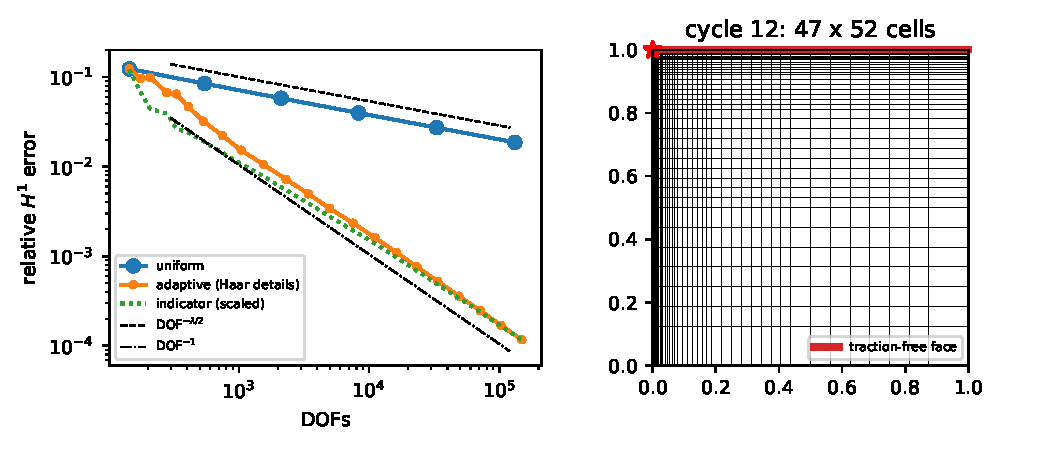
\includegraphics[width=0.8\textwidth]{../figures/elasticity_traction.pdf}
\caption{Corner singularity at the end of a traction-free face (red edge; the star marks the singular
point). Left: error versus number of unknowns. Right: grid generated after 12 refinement cycles.}\label{fig:trac}
\end{figure}

To put these numbers in context, we solved the same problem with biquadratic ($Q_2$) finite elements on
exactly the same grids, with the same type of solver: conjugate gradients preconditioned by fast
diagonalization (Table~\ref{tab:q2} and Fig.~\ref{fig:q2}). On a given grid, $Q_2$ is about 1.3 times more
accurate, but it has four times as many unknowns. At equal accuracy, the collocation method needs a quarter of the unknowns. In our implementation and on
our hardware this translated into about 2.5 to 3 times less end-to-end time including assembly (about 1.4
times without it) and about 40\% less memory. These time and memory factors depend on implementation and
hardware; the factor in unknowns does not. A sparse direct solver is one to two orders of magnitude slower
than either iterative solver, so much of the speed-up often reported for structured methods comes from the
solver. \todo{AMG baseline pending: \texttt{pip install pyamg}, then run E13 (see README).}


\begin{table}[t]\centering\small
\caption{Collocation versus $Q_2$ finite elements on identical grids (every third refinement cycle).
Memory counts operators, factorizations and Krylov vectors.}\label{tab:q2}
\textit{(a) IHWC collocation: GMRES with the FDM preconditioner}\\[2pt]
\begin{tabular}{rr c ccc}
\toprule
cycle & unknowns & $e_{H^1}$ & setup (s) & solve (s) & MB\\
\midrule
0 & 144 & $1.23{\times}10^{-1}$ & 0.00 & 0.00 & 0.3\\
3 & 280 & $6.68{\times}10^{-2}$ & 0.00 & 0.01 & 0.4\\
6 & 532 & $3.22{\times}10^{-2}$ & 0.00 & 0.01 & 0.6\\
9 & 1550 & $1.05{\times}10^{-2}$ & 0.00 & 0.01 & 1.3\\
12 & 4982 & $3.42{\times}10^{-3}$ & 0.01 & 0.01 & 3.9\\
15 & 16182 & $1.11{\times}10^{-3}$ & 0.02 & 0.04 & 12.3\\
18 & 48960 & $3.59{\times}10^{-4}$ & 0.06 & 0.13 & 37.0\\
21 & 149008 & $1.17{\times}10^{-4}$ & 0.21 & 0.48 & 112.3\\
22 & 215644 & $8.03{\times}10^{-5}$ & 0.44 & 0.78 & 162.5\\
\bottomrule
\end{tabular}

\medskip
\textit{(b) $Q_2$ finite elements on the same grids, same cycles (rows) as in (a): CG with the FDM preconditioner, and sparse direct solve}\\[2pt]
\begin{tabular}{r c cccc}
\toprule
unknowns & $e_{H^1}$ & asm.\ (s) & CG (s) & MB & direct (s)\\
\midrule
480 & $7.22{\times}10^{-2}$ & 0.00 & 0.00 & 0.2 & 0.00\\
988 & $5.39{\times}10^{-2}$ & 0.01 & 0.00 & 0.3 & 0.00\\
1944 & $2.61{\times}10^{-2}$ & 0.01 & 0.00 & 0.7 & 0.02\\
5880 & $8.43{\times}10^{-3}$ & 0.02 & 0.01 & 2.0 & 0.06\\
19344 & $2.73{\times}10^{-3}$ & 0.04 & 0.03 & 6.8 & 0.51\\
63664 & $8.80{\times}10^{-4}$ & 0.13 & 0.09 & 22.7 & 3.08\\
193980 & $2.84{\times}10^{-4}$ & 0.39 & 0.32 & 69.4 & 20.49\\
592780 & $9.21{\times}10^{-5}$ & 1.54 & 1.19 & 212.6 & --\\
858676 & $6.33{\times}10^{-5}$ & 2.10 & 2.18 & 308.2 & --\\
\bottomrule
\end{tabular}

\end{table}
\begin{figure}[t]\centering
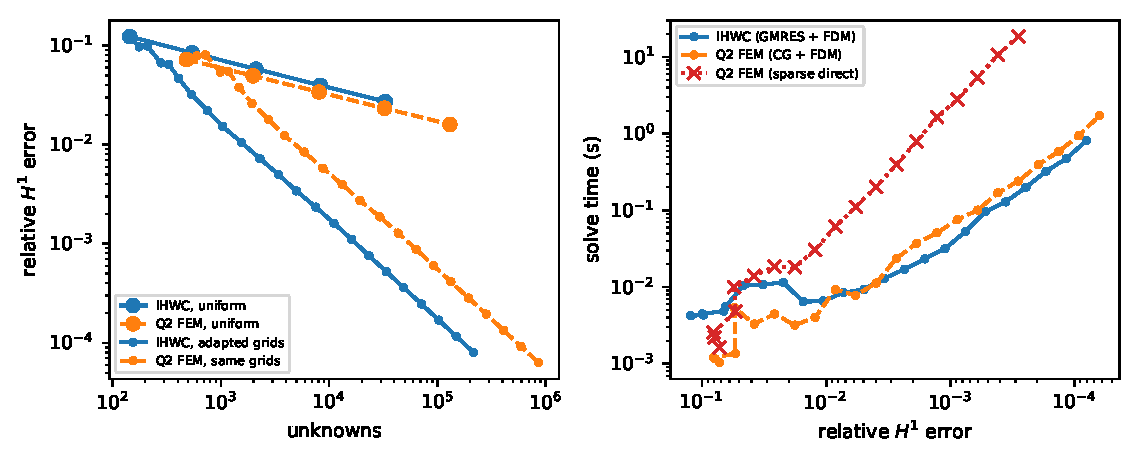
\includegraphics[width=0.9\textwidth]{../figures/ihwc_vs_q2.pdf}
\caption{Collocation versus $Q_2$ finite elements on identical grids. Left: error versus number of
unknowns. Right: solve time versus error.}\label{fig:q2}
\end{figure}

\subsection{Phase field: how many nodes does an interface need?}\label{sec:sharp}
Across an interface, $u$ goes from $-0.76$ to $0.76$ over a distance of $2\sqrt2\varepsilon$, so we measure
resolution in nodes per $\sqrt2\varepsilon$. For a planar interface solved exactly on discrete grids
(Fig.~\ref{fig:res}), plain HWCM is about twice as accurate as the standard three-point difference at every
resolution. The fourth-order operator pays off from about 1.5 nodes per $\sqrt2\varepsilon$. At 3.6 nodes it
is 25 times more accurate than finite differences, and at 7.2 nodes 110 times.

\begin{figure}[t]\centering
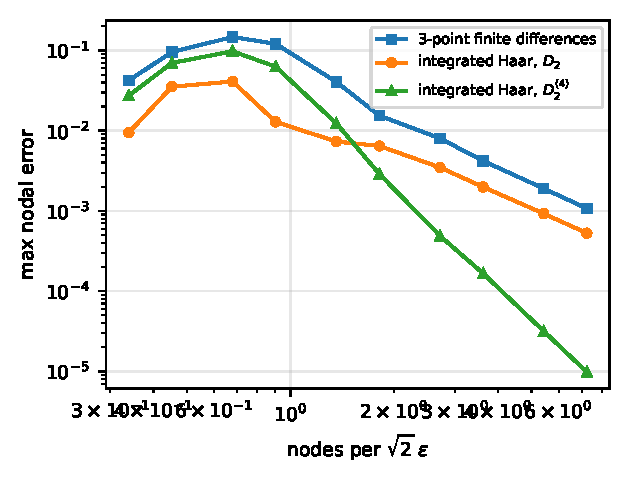
\includegraphics[width=0.5\textwidth]{../figures/interface_resolution.pdf}
\caption{Planar interface ($\varepsilon=0.01$): maximum nodal error versus nodes per $\sqrt2\varepsilon$ (data in Table~S5).}\label{fig:res}
\end{figure}

For the Allen--Cahn six-fold star with $\varepsilon=0.004$, evolving under curvature flow, a $1024^2$
computation serves as the reference (Fig.~\ref{fig:star} and Table~\ref{tab:star}). On $256^2$, which gives
only 1.45 nodes per $\sqrt2\varepsilon$, the sharp tips move too slowly with $D_2$, while $D_2^{(4)}$ follows
the reference. $D_2^{(4)}$ on $256^2$ is as accurate in area as $D_2$ on $512^2$, with a quarter of the
unknowns, and on $512^2$ it is 16 times more accurate than $D_2$.

\begin{figure}[t]\centering
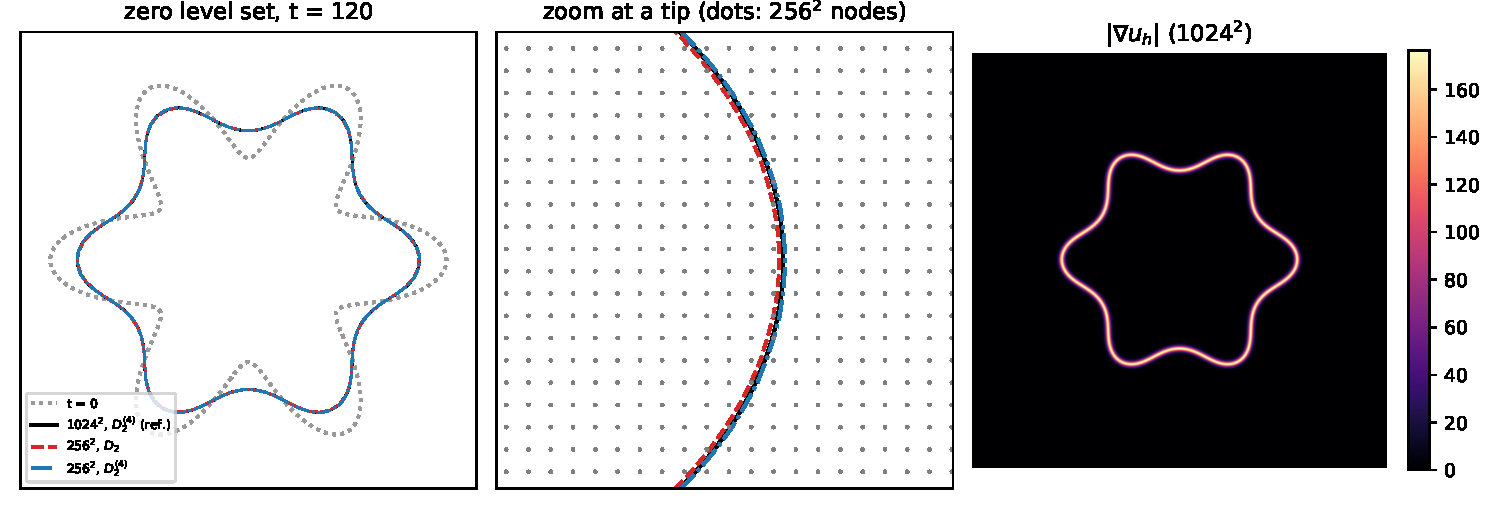
\includegraphics[width=\textwidth]{../figures/allen_cahn_star.pdf}
\caption{Allen--Cahn star, $\varepsilon=0.004$. Left: zero level sets at $t=0$ and $t=120$. Middle: zoom at
a tip, with the $256^2$ grid nodes. Right: gradient magnitude of the reference solution.}\label{fig:star}
\end{figure}
\begin{table}[t]\centering\small
\caption{Allen--Cahn star ($\varepsilon=0.004$): maximum nodal error and area error against the $1024^2$
reference, and cost per step.}\label{tab:star}
\begin{tabular}{l rcc c}
\toprule
run & unknowns & max error vs.\ ref. & area error & CPU time/step\\
\midrule
$256^2$, $D_2$ & 65536 & $1.36\times10^{-1}$ & $2.43\times10^{-4}$ & 1.6 ms\\
$256^2$, $D_2^{(4)}$ & 65536 & $5.27\times10^{-2}$ & $6.07\times10^{-5}$ & 1.4 ms\\
$512^2$, $D_2$ & 262144 & $4.12\times10^{-2}$ & $6.88\times10^{-5}$ & 9.5 ms\\
$512^2$, $D_2^{(4)}$ & 262144 & $2.63\times10^{-3}$ & $4.23\times10^{-6}$ & 8.6 ms\\
$1024^2$, $D_2^{(4)}$ (ref.) & 1048576 & -- & -- & 106 ms\\
\bottomrule
\end{tabular}

\end{table}

The most demanding case is Cahn--Hilliard with $\varepsilon=0.0015$ on $1024^2$, which gives 2.2 nodes per
$\sqrt2\varepsilon$; the whole interface spans about four nodes. With stabilized SAV ($S=4$), mass is
conserved to $10^{-17}$, both the modified and the physical energy decrease, $|u|$ stays below 1.03, and the
nodal profile across an interface coincides with the exact $\tanh$ profile. The largest computed gradient,
467, matches the exact value $1/(\sqrt2\varepsilon)=471$ (Fig.~\ref{fig:chsharp} and Table~\ref{tab:chsharp}).

\begin{figure}[t]\centering
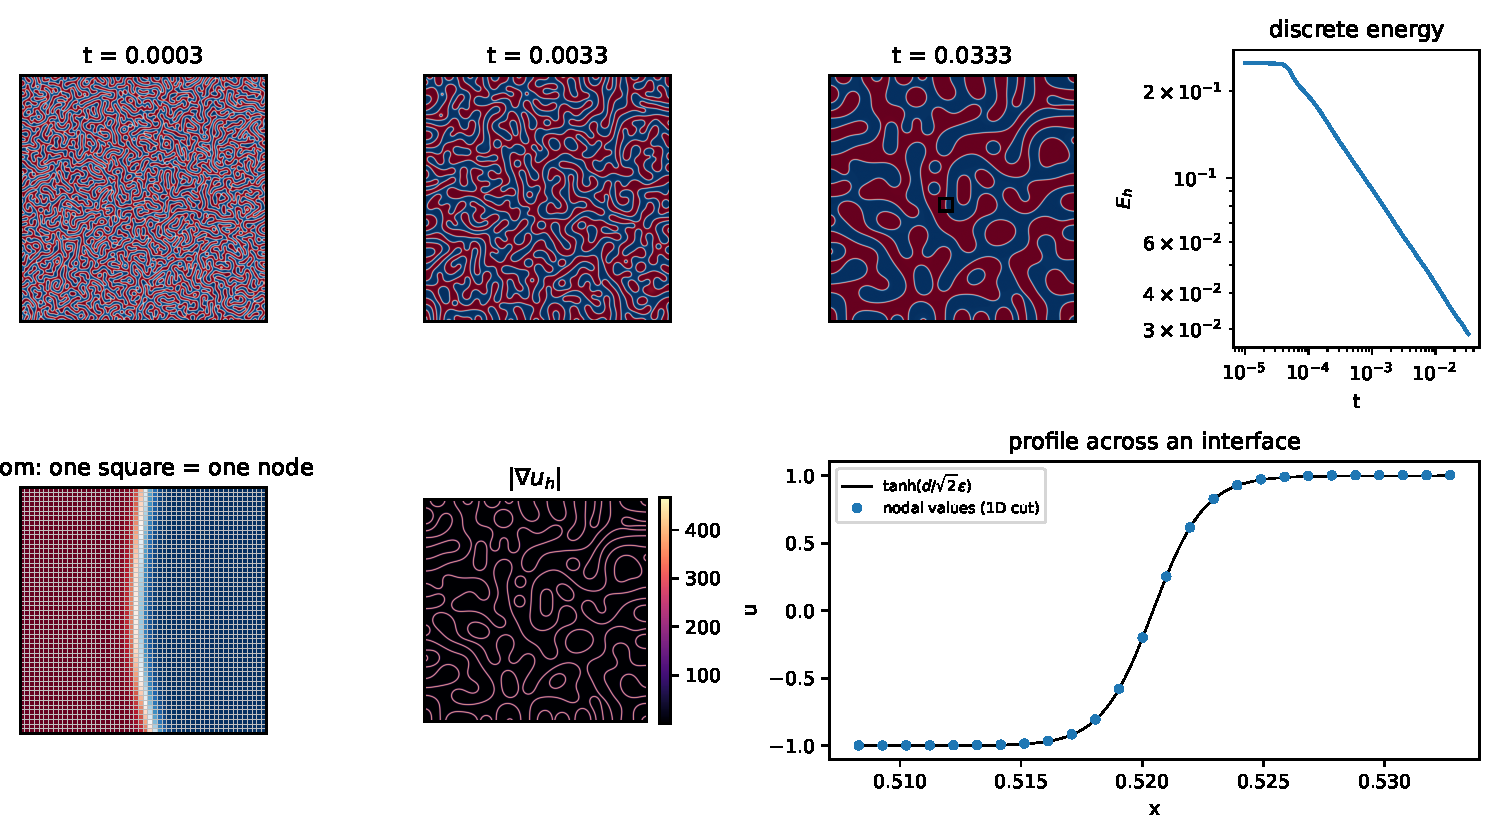
\includegraphics[width=\textwidth]{../figures/cahn_hilliard_sharp.pdf}
\caption{Cahn--Hilliard with $\varepsilon=0.0015$ on $1024^2$. Top: concentration at three times and
discrete energy. Bottom: zoom in which each square is one node; gradient magnitude; nodal values across
an interface compared with the $\tanh$ profile.}\label{fig:chsharp}
\end{figure}
\begin{table}[t]\centering\small
\caption{Cahn--Hilliard with $\varepsilon=0.0015$ on $1024^2$, stabilized SAV ($S=4$).}\label{tab:chsharp}
\begin{tabular}{p{7.2cm} c}
\toprule
quantity & value\\
\midrule
grid and $\varepsilon$ & $1024^2$, 0.0015\\
nodes per $\sqrt2\varepsilon$ & 2.17\\
time steps & 1500$\times$$2{\times}10^{-7}$, 1500$\times$$2{\times}10^{-6}$, 1500$\times$$2{\times}10^{-5}$\\
largest mass deviation & $6.49{\times}10^{-18}$\\
largest step change of the modified energy & $-7.20{\times}10^{-8}$\\
largest change of $E_h$ between samples & $-3.37{\times}10^{-5}$\\
largest $|\nabla u_h|$ / planar-interface value $1/(\sqrt2\varepsilon)$ & 467 / 471\\
largest $|u_h|$ & 1.028\\
CPU time per step (one core) & 101 ms\\
\bottomrule
\end{tabular}

\end{table}
\begin{table}[t]\centering\small
\caption{Plain ($S=0$) versus stabilized ($S=4$) SAV for $\varepsilon=0.0015$: 150 steps from $t=0.0033$.}\label{tab:savstab}
\begin{tabular}{cc cccc}
\toprule
$S$ & $\Delta t$ & $\max|u_h|$ & $E_h$ (start $\to$ end) & $\xi$ & max $\Delta\tilde E$\\
\midrule
0 & $2{\times}10^{-5}$ & 77.33 & 0.062 $\to$ 503.681 & -0.00003 & $-4.59{\times}10^{-5}$\\
0 & $5{\times}10^{-6}$ & 122.58 & 0.062 $\to$ 801.433 & -0.00002 & $-3.23{\times}10^{-5}$\\
4 & $2{\times}10^{-5}$ & 1.04 & 0.062 $\to$ 0.050 & 1.00002 & $-5.02{\times}10^{-5}$\\
4 & $5{\times}10^{-6}$ & 1.04 & 0.062 $\to$ 0.058 & 1.00000 & $-2.27{\times}10^{-5}$\\
\bottomrule
\end{tabular}

\end{table}

\subsection{When not to use the method}\label{sec:compare}
Because every uniform-grid operator considered here is diagonalized by the same cosine transform, we
could compare five of them within the identical solver: the three-point difference, $D_2$, $D_2^{(4)}$,
the classical compact (Pad\'e) scheme, and the cosine pseudo-spectral method (Fig.~\ref{fig:compare} and
Table~S15). Plain HWCM beats the three-point difference by a factor of two, and the compact scheme is about
1.4 times more accurate than $D_2^{(4)}$. For smooth problems on uniform boxes with zero-flux or periodic
conditions, however, the pseudo-spectral method is far more accurate than all others. For such problems we
recommend pseudo-spectral methods. The strength of the present method lies in graded and adaptive grids,
prescribed values and tractions, and singular solutions. The elastostatic formulation is also not robust
as Poisson's ratio approaches one half (Tables~S1 and~S2).

\begin{figure}[t]\centering
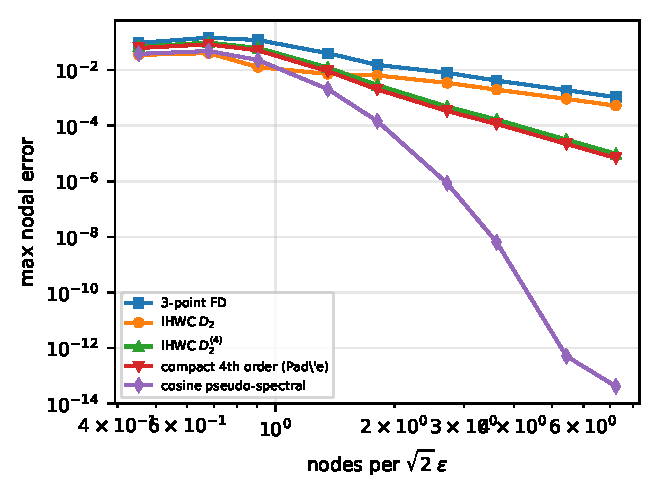
\includegraphics[width=0.5\textwidth]{../figures/scheme_comparison.pdf}
\caption{Planar interface: maximum nodal error versus resolution for five operators.}\label{fig:compare}
\end{figure}

\subsection{Performance}
A phase-field time step costs $O(N^d\log N)$ operations with fast cosine transforms. On one CPU core this
amounts to between $10^7$ and $3\times10^7$ unknowns per second (Table~\ref{tab:perf}). Absolute timings
depend on the hardware; the complexity does not. \todo{GPU columns pending; see the GPU section of the repository README.}


\begin{table}[t]\centering\small
\caption{Time per Cahn--Hilliard time step with $D_2^{(4)}$.}\label{tab:perf}
\textit{(a) CPU, double precision (ms per step)}\\[2pt]
\begin{tabular}{rr r cc}
\toprule
$d$ & $N$ & unknowns & GEMM & DCT\\
\midrule
2 & 128 & 16384 & 0.77 & 0.34\\
2 & 256 & 65536 & 2.25 & 1.55\\
2 & 512 & 262144 & 12.69 & 12.02\\
2 & 1024 & 1048576 & 146.23 & 103.26\\
2 & 2048 & 4194304 & -- & 363.06\\
3 & 32 & 32768 & 0.99 & 1.06\\
3 & 64 & 262144 & 8.11 & 9.41\\
3 & 128 & 2097152 & 191.31 & 189.90\\
\bottomrule
\end{tabular}

\medskip
\textit{(b) GPU (ms per step)}\\[2pt]
\begin{tabular}{rr cc cc}
\toprule
& & \multicolumn{2}{c}{double precision} & \multicolumn{2}{c}{single precision}\\
$d$ & $N$ & GEMM & DCT & GEMM & DCT\\
\midrule
2 & 128 & 1.10 & 2.13 & 1.18 & 2.17\\
2 & 256 & 3.14 & 2.59 & 3.29 & 2.18\\
2 & 512 & 13.98 & 2.89 & 11.21 & 2.88\\
2 & 1024 & 75.91 & 10.63 & 76.42 & 10.62\\
2 & 2048 & 589.88 & 44.33 & 591.10 & 44.18\\
3 & 32 & 1.46 & 2.93 & 1.80 & 2.94\\
3 & 64 & 3.35 & 3.66 & 3.42 & 3.63\\
3 & 128 & 35.14 & 31.91 & 34.97 & 32.05\\
\bottomrule
\end{tabular}

\end{table}

%==========================================================================
\section{Practical guidelines}\label{sec:guide}
%==========================================================================
Table~\ref{tab:guide} summarizes the choices that worked in our computations.

\begin{table}[t]\centering\small
\caption{Practical recommendations.}\label{tab:guide}
\begin{tabular}{p{3.3cm}p{10.6cm}}
\toprule
Decision & Recommendation\\
\midrule
Plain or corrected operator & Use $D_2^{(4)}$ for zero-flux or periodic problems, since it costs nothing extra. With general prescribed values, use $D_2$, because the correction does not raise the order there.\\
When not to use IHWC & For smooth or phase-field problems on uniform boxes with zero-flux or periodic conditions, a cosine pseudo-spectral operator is far more accurate at the same cost (Section~\ref{sec:compare}).\\
Interface resolution & Use at least 1.5 nodes per $\sqrt2\varepsilon$ with $D_2^{(4)}$. Expect a nodal error of about $10^{-3}$ at 2 to 3 nodes, and about $10^{-4}$ at 3.5 nodes (Table~S5).\\
Time stepping (AC, CH) & Use SAV-BDF2 with stabilization $S\approx4$ and monitor $\xi=r/\sqrt{E_{1,h}+C}$; if it leaves $[0.999,1.001]$, reduce $\Delta t$. Start with small steps from random initial data, and increase $\Delta t$ as the structure coarsens, restarting with BDF1 at each change.\\
Solver & On uniform grids, use cosine or sine transforms. On graded grids, use fast diagonalization with dense matrix products (Result~\ref{thm:spectrum} guarantees that it applies). For coupled systems such as elasticity, use GMRES with the block preconditioner.\\
Adaptivity at singularities & Use the Haar-detail indicator with D\"orfler parameter $\theta\approx0.6$, a neighbour ratio of at most two, and an initial grid of $8\times8$ cells.\\
Traction conditions & Collocate tractions plainly at edge midpoints, without enhancement, and use the two normal-stress conditions at traction--traction corners.\\
Near incompressibility & Avoid $\nu>0.45$ with the present formulation (Tables~S1 and~S2).\\
\bottomrule
\end{tabular}
\end{table}

%==========================================================================
\section{Limitations}\label{sec:limits}
%==========================================================================
The fast solvers require rectangular domains; the full L-shaped domain and curved boundaries need
multi-patch coupling or geometry maps. Refinement is anisotropic but not local, which costs a constant
factor of about four in cells at point singularities. Proved results and observations should be
distinguished. Proved are the three-term identity, the real spectrum on every grid, the fourth-order
correction and the symmetric structure on uniform grids, exact mass conservation, and the decay of the
modified energy on uniform grids. Observed, but not proved, are the conditioning of the eigenvectors, the
decay of the physical energy, the boundedness of $u$, the reliability of the refinement indicator, the
optimal adaptive rates, and the mesh-independent iteration counts. The last of these hold for compressible
materials only. Comparisons with adaptive isogeometric collocation and with multigrid-preconditioned finite
elements are still missing.

%==========================================================================
\section{Conclusions}
%==========================================================================
Haar wavelet collocation, rewritten in nodal form, has a second-derivative operator whose eigenvalues are
real, distinct and nonpositive on every grid. This one property makes the fastest structured solvers
applicable to any graded or adaptively refined tensor grid. It turns the dense HWCM systems into
millisecond solves, and it supports phase-field solvers that conserve mass exactly, remain energy-stable,
and resolve interfaces only a few nodes wide. For elastostatics with tractions, the method recovers optimal
convergence at corner singularities automatically. Against biquadratic finite elements on the same grids and with the same kind of solver, it needs a
quarter of the unknowns for a given accuracy.

\section*{Code and data availability}
The implementation, the tests and the scripts that produce every table and figure are available at \repo;
the version used here is the GitHub release v1.1 (\archive).
Dependencies are listed in \texttt{requirements.txt} (CPU) and \texttt{requirements-gpu.txt} (GPU).

\section*{Declaration of competing interest}
The author declares no known competing financial interests or personal relationships that could have
appeared to influence the work reported in this paper.

\begin{thebibliography}{99}
\bibitem{chen1997haar} C.F. Chen, C.H. Hsiao, Haar wavelet method for solving lumped and distributed-parameter systems, IEE Proc. Control Theory Appl. 144 (1997) 87--94.
\bibitem{lepik2005numerical} \"U. Lepik, Numerical solution of differential equations using Haar wavelets, Math. Comput. Simul. 68 (2005) 127--143.
\bibitem{lepik2011solving} \"U. Lepik, Solving PDEs with the aid of two-dimensional Haar wavelets, Comput. Math. Appl. 61 (2011) 1873--1879.
\bibitem{lepik2014book} \"U. Lepik, H. Hein, Haar Wavelets: With Applications, Springer, Cham, 2014.
\bibitem{majak2015accuracy} J. Majak, B. Shvartsman, K. Karjust, M. Mikola, A. Haavaj\~oe, M. Pohlak, On the accuracy of the Haar wavelet discretization method, Compos. B Eng. 80 (2015) 321--327.
\bibitem{majak2015convergence} J. Majak, B.S. Shvartsman, M. Kirs, M. Pohlak, H. Herranen, Convergence theorem for the Haar wavelet based discretization method, Compos. Struct. 126 (2015) 227--232.
\bibitem{majak2018higher} J. Majak, M. Pohlak, K. Karjust, M. Eerme, J. Kurnitski, B.S. Shvartsman, New higher order Haar wavelet method: Application to FGM structures, Compos. Struct. 201 (2018) 72--78.
\bibitem{ratas2021solving} M. Ratas, J. Majak, A. Salupere, Solving nonlinear boundary value problems using the higher order Haar wavelet method, Mathematics 9 (2021) 2809.
\bibitem{dubeau2004nonuniform} F. Dubeau, S. Elmejdani, R. Ksantini, Non-uniform Haar wavelets, Appl. Math. Comput. 159 (2004) 675--693.
\bibitem{lepik2008nonuniform} \"U. Lepik, Solving integral and differential equations by the aid of non-uniform Haar wavelets, Appl. Math. Comput. 198 (2008) 326--332.
\bibitem{oruc2019nonuniform} \"O. Oru\c{c}, A non-uniform Haar wavelet method for numerically solving two-dimensional convection-dominated equations and two-dimensional near singular elliptic equations, Comput. Math. Appl. 77 (2019) 1799--1820.
\bibitem{houstis1988quadratic} E.N. Houstis, C.C. Christara, J.R. Rice, Quadratic-spline collocation methods for two-point boundary value problems, Int. J. Numer. Methods Eng. 26 (1988) 935--952.
\bibitem{christara1994quadratic} C.C. Christara, Quadratic spline collocation methods for elliptic partial differential equations, BIT 34 (1994) 33--61.
\bibitem{christara2006optimal} C.C. Christara, K.S. Ng, Optimal quadratic and cubic spline collocation on nonuniform partitions, Computing 76 (2006) 227--257.
\bibitem{christara2006adaptive} C.C. Christara, K.S. Ng, Adaptive techniques for spline collocation, Computing 76 (2006) 259--277.
\bibitem{christara2002fast} C.C. Christara, K.S. Ng, Fast Fourier transform solvers and preconditioners for quadratic spline collocation, BIT 42 (2002) 702--739.
\bibitem{auricchio2010isogeometric} F. Auricchio, L. Beir\~ao da Veiga, T.J.R. Hughes, A. Reali, G. Sangalli, Isogeometric collocation methods, Math. Models Methods Appl. Sci. 20 (2010) 2075--2107.
\bibitem{schillinger2013isogeometric} D. Schillinger, J.A. Evans, A. Reali, M.A. Scott, T.J.R. Hughes, Isogeometric collocation: Cost comparison with Galerkin methods and extension to adaptive hierarchical NURBS discretizations, Comput. Methods Appl. Mech. Engrg. 267 (2013) 170--232.
\bibitem{delorenzis2015isogeometric} L. De Lorenzis, J.A. Evans, T.J.R. Hughes, A. Reali, Isogeometric collocation: Neumann boundary conditions and contact, Comput. Methods Appl. Mech. Engrg. 284 (2015) 21--54.
\bibitem{lynch1964direct} R.E. Lynch, J.R. Rice, D.H. Thomas, Direct solution of partial difference equations by tensor product methods, Numer. Math. 6 (1964) 185--199.
\bibitem{bartels1972solution} R.H. Bartels, G.W. Stewart, Solution of the matrix equation $AX+XB=C$, Commun. ACM 15 (1972) 820--826.
\bibitem{sangalli2016isogeometric} G. Sangalli, M. Tani, Isogeometric preconditioners based on fast solvers for the Sylvester equation, SIAM J. Sci. Comput. 38 (2016) A3644--A3671.
\bibitem{shen2018scalar} J. Shen, J. Xu, J. Yang, The scalar auxiliary variable (SAV) approach for gradient flows, J. Comput. Phys. 353 (2018) 407--416.
\bibitem{gantmacher2002oscillation} F.R. Gantmacher, M.G. Krein, Oscillation Matrices and Kernels and Small Vibrations of Mechanical Systems, revised ed., AMS Chelsea Publishing, Providence, RI, 2002.
\bibitem{dorfler1996convergent} W. D\"orfler, A convergent adaptive algorithm for Poisson's equation, SIAM J. Numer. Anal. 33 (1996) 1106--1124.
\bibitem{williams1952stress} M.L. Williams, Stress singularities resulting from various boundary conditions in angular corners of plates in extension, J. Appl. Mech. 19 (1952) 526--528.
\bibitem{dyksen1987tensor} W.R. Dyksen, Tensor product generalized ADI methods for separable elliptic problems, SIAM J. Numer. Anal. 24 (1987) 59--76.
\bibitem{sun1999spectral} W. Sun, Spectral analysis of Hermite cubic spline collocation systems, SIAM J. Numer. Anal. 36 (1999) 1962--1975.
\bibitem{bialecki1995matrix} B. Bialecki, G. Fairweather, Matrix decomposition algorithms in orthogonal spline collocation for separable elliptic boundary value problems, SIAM J. Sci. Comput. 16 (1995) 330--347.
\bibitem{bialecki2011matrix} B. Bialecki, G. Fairweather, A. Karageorghis, Matrix decomposition algorithms for elliptic boundary value problems: a survey, Numer. Algorithms 56 (2011) 253--295.
\end{thebibliography}

\end{document}
